\section{Nivel 1 --- Control supervisor (DEDS)}

\begin{frame}{Twistlocks}
  \begin{columns}[T]
    \begin{column}{0.5\textwidth}
      Cuatro estados: \texttt{VACIO} $\to$ \texttt{CERRANDO} $\to$ \texttt{CARGADO} $\to$
      \texttt{ABRIENDO}.
      \begin{itemize}
        \item Toma/libera la carga sólo con el spreader \textbf{apoyado} (interlock).
        \item \textbf{Estima la masa} del contenedor con la celda de carga.
        \item Detecta \textbf{sobrecarga} y limita la velocidad por curva de potencia.
          \begin{equation*}
        v_{h,lim}({m}_l) = 
        \begin{cases} 
            v_{h\max} & \text{si } {m}_l < 32500 kg \\
            \frac{P_{h\ nom}}{{m}_l \, g} & \text{si } {m}_l \ge 32500 kg
        \end{cases}
    \end{equation*}
      \end{itemize}
    \end{column}
    \begin{column}{0.5\textwidth}
      \centering
      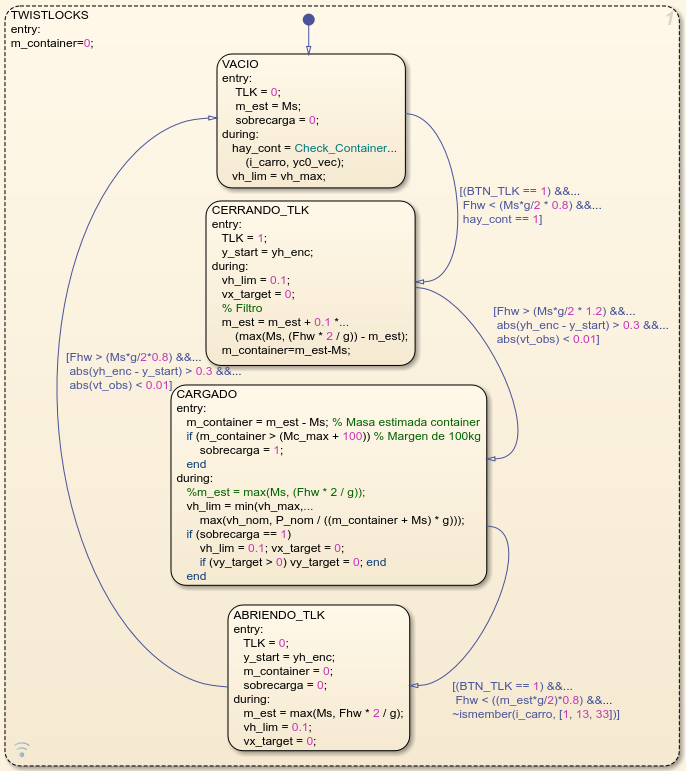
\includegraphics[height=0.95\textheight]{nivel_1/twistlocks_p.png}
    \end{column}
  \end{columns}
\end{frame}

\begin{frame}{Análisis espacial}
      \centering
      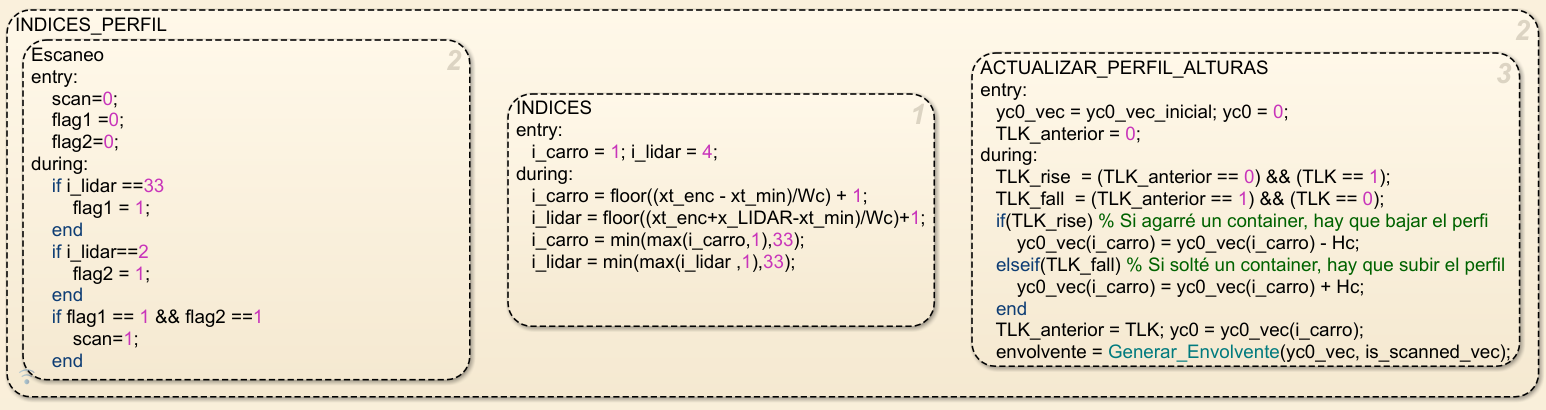
\includegraphics[width=\linewidth]{nivel_1/indices_perfil_p.png}
\end{frame}

\begin{frame}{Límites suaves de velocidad}
      \begin{columns}[T]
        \begin{column}{0.48\textwidth}
          \centering
          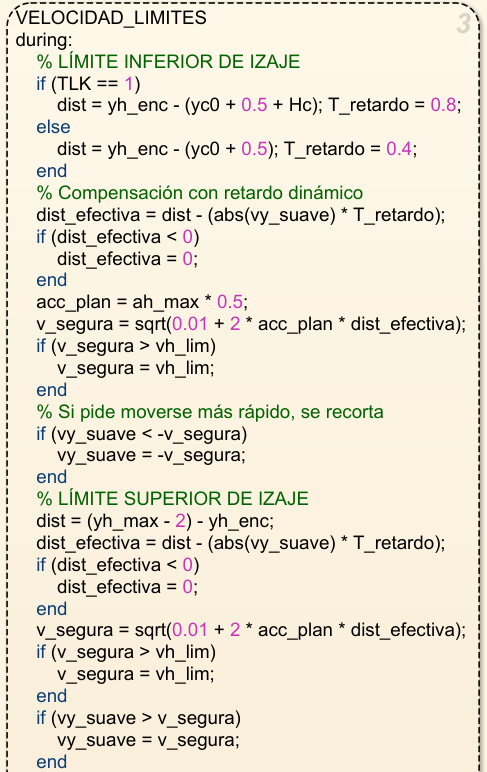
\includegraphics[width=0.7\textwidth]{nivel_1/limites1.png}
        \end{column}
        \begin{column}{0.48\textwidth}
          \centering
          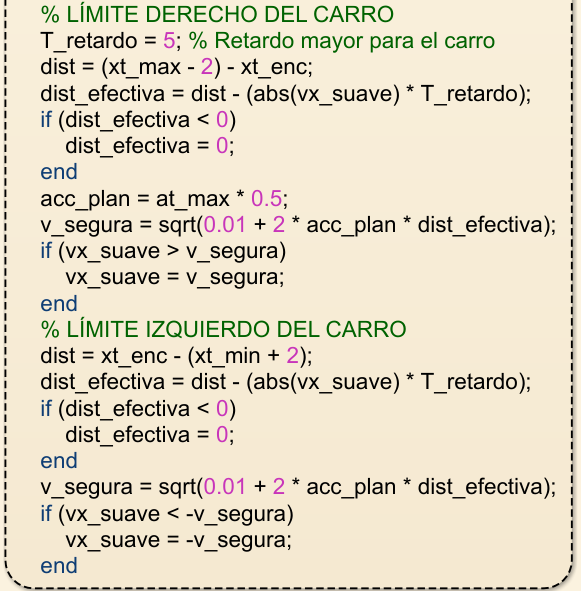
\includegraphics[width=\textwidth]{nivel_1/limites2.png}
        \end{column}
      \end{columns}
\end{frame}

\begin{frame}{Suavizado y watchdog}
  \begin{columns}[T]
     \begin{column}{0.5\textwidth}
      \begin{block}{Suavizado}
        Convierte consignas crudas en $v_{suave}$.
      \end{block}
      \centering
      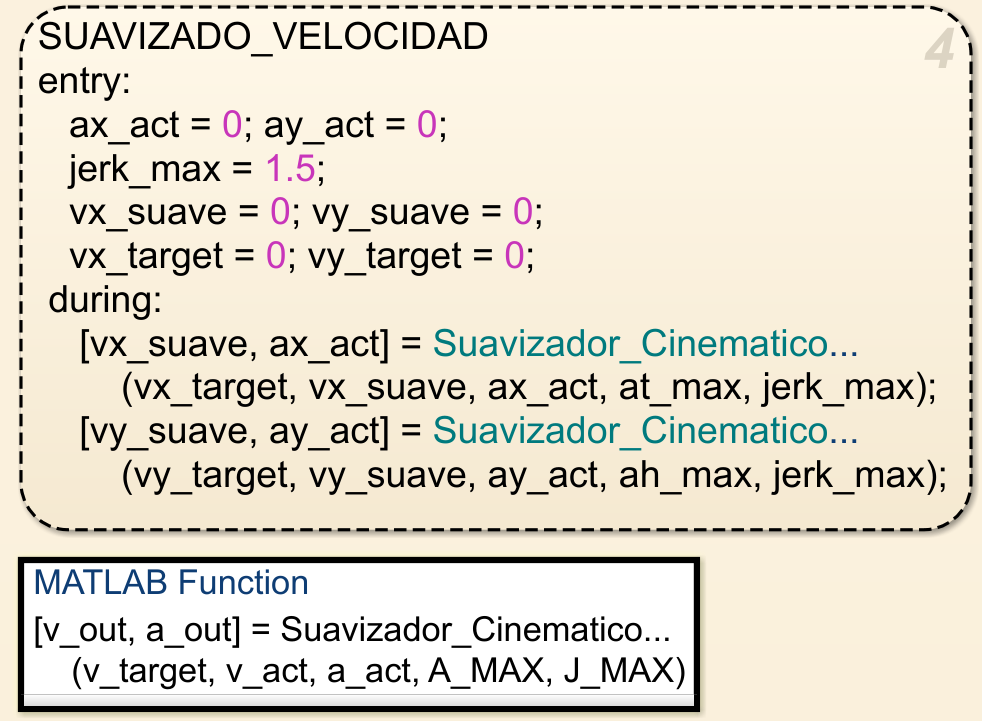
\includegraphics[width=\linewidth]{nivel_1/suavizado_p.png}
    \end{column}
    \begin{column}{0.5\textwidth}
      \begin{block}{Watchdog}
        Genera un heartbeat cada cierto tiempo que recibe el Nivel 0.
      \end{block}
      \centering
      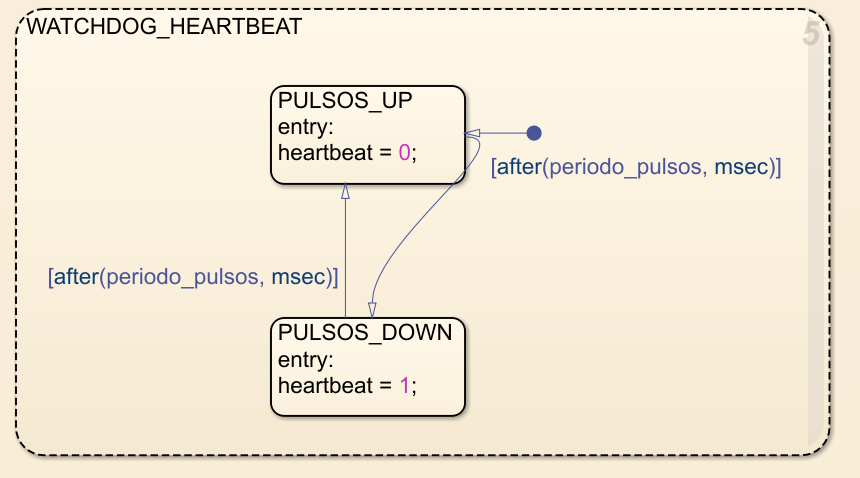
\includegraphics[width=\linewidth]{nivel_1/watchdog_heartbeat.png}
    \end{column}
  \end{columns}
\end{frame}
